\centerline{\bf \Huge Степень точки}

\begin{flushright}
        \scriptsize{Пора спать, бай-бай\\завтра вставать в восемь...}
\end{flushright}

\textbf{Определение.}
Степенью точки $X$ относительно окружности $\omega$ называется величина $\operatorname{Pow}(X, \omega)=d^2-R^2$, где $d-$ расстояние от точки $X$ до центра окружности, а $R$ - радиус окружности.

Если прямая, проходящая через точку $X$, пересекает $\omega$ в точках $A$ и $B$, то степень точки равна $X A \cdot X B$, взятая со знаком «+», если $X$ лежит вне $\omega$, и со знаком «-», если внутри.

\begin{figure}[h]
    \centering
    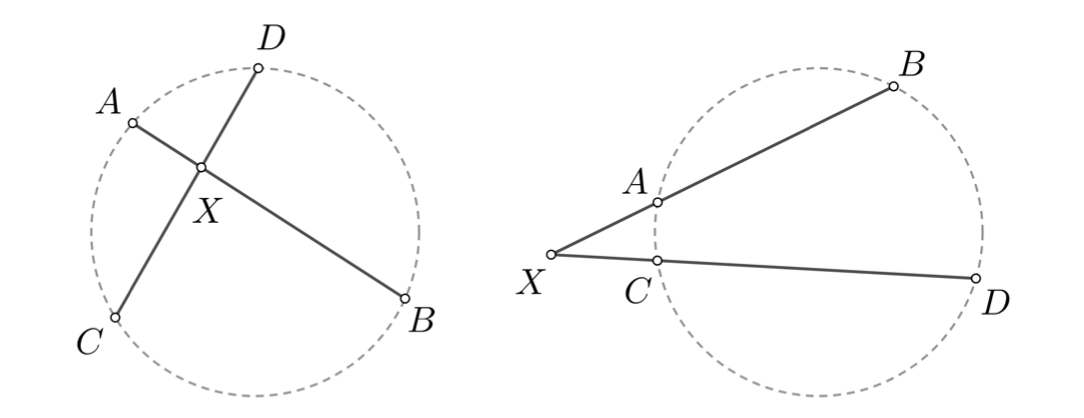
\includegraphics[width=1\linewidth]{Сборы//Зимние сборы 2026//9-10/power_point.png}
    \caption{}
    \label{fig:placeholder}
\end{figure}

\textbf{Утверждение.} Для обеих картинок сверху точки $A, B, C, D$ лежат на одной окружности тогда и только тогда, когда $X A \cdot X B=X C \cdot X D$.

Аналогичные утверждения верны, если секущую заменить на касательную.

\problem{1}
Дан четырёхугольник $A B C D$, в котором $\angle C A B=\angle D B C$ и $\angle B C A= \angle C D B$. Обозначим через $O$ его точку пересечения диагоналей. Докажите, что длины касательных из точек $B$ и $C$ к описанной окружности треугольника $A O D$ равны.

\problem{2}
В треугольнике $A B C$ проведена биссектриса $A D$. Описанные окружности треугольников $A B D$ и $A C D$ пересекают отрезки $A C$ и $A B$ в точках $E$ и $F$ соответственно. Докажите, что $B F=C E$.

\newpage

\hspace{3mm}

\problem{3}
Точка $D$ - середина стороны $B C$ треугольника $A B C$, точка $E$ - середина отрезка $D C$. Описанная окружность треугольника $A B E$ вторично пересекает сторону $A C$ в точке $F$. Докажите, что $\angle B A D=\angle D F E$.

\problem{4}
Диагонали трапеции $A B C D$ с основаниями $A D$ и $B C$ пересекаются в точке $P$. Известно, что $\angle A P B<90^{\circ}$. Докажите, что длины отрезков касательных, проведённых из точки $P$ к окружностям, построенным на отрезках $A B$ и $C D$ как на диаметрах, равны.

\problem{5}
На прямых, содержащих высоты $B B_1$ и $C C_1$ треугольника $A B C$, выбраны такие точки, что соответствующие стороны (т. е. стороны $A C$ и $A B$ ) видны из них под прямым углом. Докажите, что четыре отмеченные точки лежат на одной окружности.

\problem{6}
На плоскости даны окружность $\omega$, точка $A$, лежащая внутри $\omega$, и точка $B$, лежащая вне $\omega$. Рассматриваются всевозможные треугольники $B X Y$ такие, что точки $X$ и $Y$ лежат на $\omega$ и хорда $X Y$ проходит через точку $A$. Докажите, что центры окружностей, описанных около треугольников $B X Y$, лежат на одной прямой.

\problem{7}
Окружности $\Omega$ и $\omega$ касаются внутренним образом в точке $A$. Хорда $B C$ окружности $\Omega$ касается окружности $\omega$ в точке $D$. Докажите, что середина отрезка $A D$, центр $\omega$, точки $B$ и $C$ лежат на одной окружности.

\problem{8}
Противоположные стороны четырёхугольника, вписанного в окружность, пересекаются в точках $P$ и $Q$. Найдите длину отрезка $P Q$, если касательные к окружности, проведённые из точек $P$ и $Q$, равны $a$ и $b$ соответственно.